\documentclass[border=10pt]{standalone}
\usepackage{tikz}
\usepackage{fontspec}
\usepackage{xcolor}

% Use TeX Gyre Termes (Times clone) which is available in all TeX distributions
\setmainfont{TeX Gyre Termes}
\setsansfont{TeX Gyre Heros}
\setmonofont{TeX Gyre Cursor}

% TikZ libraries
\usetikzlibrary{shapes,arrows,positioning,calc,patterns,decorations.pathreplacing,chains,shadows}
\usetikzlibrary{shapes.geometric,shapes.symbols,shapes.misc}
\usetikzlibrary{matrix,fit,backgrounds}
\usetikzlibrary{arrows.meta}

% Custom colors
\definecolor{bertblue}{RGB}{66,133,244}
\definecolor{gptgreen}{RGB}{52,168,83}
\definecolor{vitpurple}{RGB}{142,36,245}
\definecolor{maskred}{RGB}{234,67,53}
\definecolor{clsorange}{RGB}{251,188,5}
\definecolor{darkgray}{RGB}{50,50,50}
\definecolor{unkred}{RGB}{234,67,53}
\definecolor{subwordpurple}{RGB}{142,36,245}
\definecolor{sepviolet}{RGB}{142,36,245}

% Custom commands for special tokens
\newcommand{\specialtoken}[1]{\texttt{[#1]}}
\newcommand{\cls}{\specialtoken{CLS}}
\newcommand{\sep}{\specialtoken{SEP}}
\newcommand{\mask}{\specialtoken{MASK}}
\newcommand{\pad}{\specialtoken{PAD}}
\newcommand{\unk}{\specialtoken{UNK}}
\newcommand{\sos}{\specialtoken{SOS}}
\newcommand{\eos}{\specialtoken{EOS}}

\begin{document}
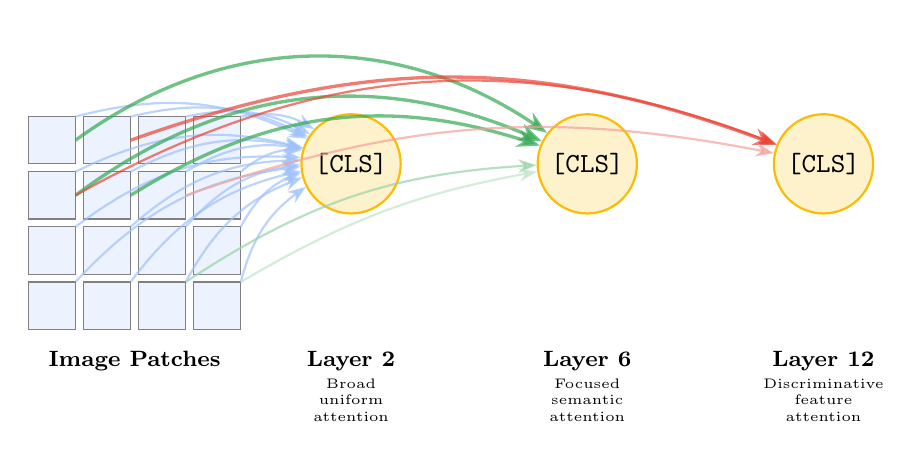
\begin{tikzpicture}[
    patch/.style={rectangle, minimum width=0.6cm, minimum height=0.6cm, draw=gray},
    clstoken/.style={circle, minimum width=0.8cm, fill=clsorange!20, draw=clsorange, thick},
    attention/.style={-{Stealth}, thick, opacity=0.7},
    layer/.style={font=\footnotesize\bfseries}
]

% Image patches grid
\foreach \x in {0,1,2,3} {
    \foreach \y in {0,1,2,3} {
        \node[patch, fill=bertblue!10] at (\x*0.7, \y*0.7 + 5) {};
    }
}

% CLS tokens for different layers
\node[clstoken] (cls1) at (3.8, 6.8) {\cls{}};
\node[clstoken] (cls2) at (6.8, 6.8) {\cls{}};
\node[clstoken] (cls3) at (9.8, 6.8) {\cls{}};

% Layer labels
\node[layer] at (1.05, 4.3) {Image Patches};
\node[layer] at (3.8, 4.3) {Layer 2};
\node[layer] at (6.8, 4.3) {Layer 6};
\node[layer] at (9.8, 4.3) {Layer 12};

% Attention patterns - Early layer (broad)
\foreach \x in {0,1,2,3} {
    \foreach \y in {0,1,2,3} {
        \draw[attention, bertblue!50] (\x*0.7 + 0.3, \y*0.7 + 5.3) to[bend left=20] (cls1);
    }
}

% Attention patterns - Middle layer (focused)
\draw[attention, gptgreen, very thick] (0.3, 6.4) to[bend left=30] (cls2);
\draw[attention, gptgreen, very thick] (1.0, 6.4) to[bend left=25] (cls2);
\draw[attention, gptgreen, very thick] (0.3, 7.1) to[bend left=35] (cls2);
\draw[attention, gptgreen!50] (1.7, 5.3) to[bend left=15] (cls2);
\draw[attention, gptgreen!30] (2.4, 5.3) to[bend left=10] (cls2);

% Attention patterns - Late layer (discriminative)
\draw[attention, maskred, very thick] (1.0, 7.1) to[bend left=20] (cls3);
\draw[attention, maskred, thick] (0.3, 6.4) to[bend left=25] (cls3);
\draw[attention, maskred!50] (1.7, 6.4) to[bend left=15] (cls3);

% Labels
\node[font=\tiny, align=center] at (3.8, 3.8) {Broad\\uniform\\attention};
\node[font=\tiny, align=center] at (6.8, 3.8) {Focused\\semantic\\attention};
\node[font=\tiny, align=center] at (9.8, 3.8) {Discriminative\\feature\\attention};

\end{tikzpicture}
\end{document}